\documentclass[12pt, twoside]{article}
\usepackage[letterpaper, margin=1in, headsep=0.2in]{geometry}
\setlength{\headheight}{0.6in}
%\usepackage[english]{babel}
\usepackage[utf8]{inputenc}
\usepackage{microtype}
\usepackage{amsmath}
\usepackage{amssymb}
%\usepackage{amsfonts}
\usepackage{siunitx} %units in math. eg 20\milli\meter
\usepackage{yhmath} % for arcs, overparenth command
\usepackage{tikz} %graphics
\usetikzlibrary{quotes, angles}
\usepackage{graphicx} %consider setting \graphicspath{{images/}}
\usepackage{parskip} %no paragraph indent
\usepackage{enumitem}
\usepackage{multicol}
\usepackage{venndiagram}

\usepackage{fancyhdr}
\pagestyle{fancy}
\fancyhf{}
\renewcommand{\headrulewidth}{0pt} % disable the underline of the header
\raggedbottom
\hfuzz=2mm %suppresses overfull box warnings

\usepackage{hyperref}

\fancyhead[LE]{\thepage}
\fancyhead[RO]{\thepage \\ Name: \hspace{4cm} \,\\}
\fancyhead[LO]{BECA / Dr. Huson / Geometry\\*  Unit 6: Analytic geometry\\* 29 November 2022}

\begin{document}

\subsubsection*{6.5 Classwork: Tangent function, slope \hfill CCSS.HSG.SRT.C.8}
\begin{enumerate}
\item Do Now: A vector from the origin $\overrightarrow{OA}$ is shown rotated counterclockwise around $O$.
  \begin{multicols}{2}
        \begin{enumerate}
        \item Using a protractor, measure the angle of rotation.
        \item Write down the slope of $\overrightarrow{OA'}$.
        \item Mark and label the point $B(4,-3)$. Draw $\overrightarrow{OB}$.
        \item Write down the slope of $\overrightarrow{OB}$.
        \item What is the product of the slopes of $\overrightarrow{OA'}$ and $\overrightarrow{OB}$?
      \end{enumerate}
      \begin{center}
      \begin{tikzpicture}[scale=1]
      \draw [help lines] (0,-5) grid (5,5);
      \draw [<->] (-0.8,0) -- (5.4,0) node [right] {$x$};
      \draw [thick, <->] (0,-5.4)--(0,5.4) node [above] {$y$};
      \foreach \x in {0,1,2,3,4,5}
        \draw[shift={(\x,0)},color=black] (0pt,-3pt) -- (0pt,3pt) node[below=5pt]  {$\x$};
      \foreach \y in {-5,...,-1,1,2,3,4,5}
        \draw[shift={(0,\y)},color=black] (-3pt,0pt) -- (3pt,0pt) node[left=5pt]  {$\y$};
      %\draw [dashed] (0,0) circle [radius=5cm];
      \draw [dashed] (-100:5) arc (-100:100:5);
      \node at (0,0)[above left]{$O$};
      \draw [line width=2pt, ->] (0,0)--(5,0) node [above left] {$A$};
      \draw [line width=2pt, ->] (0,0)--(3,4) node [above right] {$A'$};
    \end{tikzpicture}
  \end{center}
\end{multicols}

\item Complete the table mapping angle of rotation onto slope. (six entries)\\
      \begin{tikzpicture}[scale=0.5]
      \draw [help lines] (-13,0) grid (13,13);
      \draw [thick, <->] (-13.4,0) -- (13.4,0) node [right] {$x$};
      \draw [thick, <->] (0,0)--(0,13.4) node [above] {$y$};
      \foreach \x in {-13,-11,...,13}
        \draw[shift={(\x,0)},color=black] (0pt,-3pt) -- (0pt,3pt) node[below=5pt]  {$\x$};
      \foreach \y in {1,...,13}
        \draw[shift={(0,\y)},color=black] (-3pt,0pt) -- (3pt,0pt) node[left=5pt]  {$\y$};
      %\draw [dashed] (0,0) circle [radius=5cm];
      \draw [dashed] (0:13) arc (0:180:13);
      \draw [line width=2pt, ->] (0,0)--(13,0) node [above left] {$A$};
      \draw [fill] (12,5) circle [radius=0.1cm] node[above right]{$(12,5)$};
      \draw [fill] (5,12) circle [radius=0.1cm] node[above]{$(5,12)$};
      \draw [fill] (-5,12) circle [radius=0.1cm] node[above]{$(-5,12)$};
      \draw [fill] (9,9) circle [radius=0.1cm] node[above right]{$(9,9)$};
      \draw [fill] (0,13) circle [radius=0.1cm] node[above right]{$(0,13)$};

      \draw [thick] (-20,12) node [above right] {angle} -- (-14,12) node [above left] {slope};
      \draw [thick] (-17,13)--(-17,-1);
      \node at (-19,11){$0$};
      \node at (-15,9){$5/12$};
    \end{tikzpicture}

\newpage
  \item Use a calculator. Express the result to the nearest thousandth.\vspace{.5cm}
    \begin{multicols}{2}
      \begin{enumerate}
        \item $\tan 45^\circ = $ \vspace{1cm}
        \item $\tan 30^\circ =$
        \item $\tan 15^\circ = $ \vspace{1cm}
        \item $\tan 65^\circ =$
      \end{enumerate}
    \end{multicols} \vspace{0.5cm}

    \item \begin{enumerate}
      \item Graph and label $\triangle ABC$ with $A(0,0)$, $B(7,4)$, and $C(7,0)$.
      \begin{center}
        \begin{tikzpicture}%[scale=.635]
          \draw [help lines] (0,0) grid (10,6);
          \draw [thick, ->] (0,0) -- (10.4,0) node [below right] {$x$};
          \draw [thick, ->] (0,0)--(0,6.4) node [left] {$y$};
        \end{tikzpicture}
      \end{center}
      \item Find the slope and $y$-intercept of the line $\overleftrightarrow{AB}$.
        \begin{multicols}{2}
          $m_{AB}=$ \\
          $b_{AB}=$
        \end{multicols} \vspace{0.5cm}
      \item Write down the equation of each line. \\[0.5cm]
        $\overleftrightarrow{AB}$: \hfill
        $\overleftrightarrow{BC}$: \hfill
        $\overleftrightarrow{AC}$: \hspace{2cm}
      \vspace{2cm}
      \item Find the measure of $\angle BAC=\theta$ in degrees with a protractor. \vspace{0.5cm}
      \item Find the slope of $\overleftrightarrow{AB}$ using the tangent function.\\[0.5cm]
      $\displaystyle \tan(\theta)=$
      \vspace{2cm}
    \end{enumerate}

\newpage
\item Do Now: Write down the slope perpendicular to the given slope. (negative reciprocal) \vspace{0.5cm}
\begin{enumerate}
  \begin{multicols}{2}
  \item   $m= \frac{1}{3} \hspace{1cm} m_{\perp} = $
  \item   $m= -0.8 \hspace{1cm} m_{\perp} = $ 
  \end{multicols}
\end{enumerate}

\item $\triangle ABC$ is shown with $m\angle C=90^\circ$ and the lengths of the triangle's sides are $BC=8$, $AC=15$, and $AB=17$. (not drawn to scale)
  \begin{multicols}{2}
    \begin{enumerate}
      \item How long is the \emph{hypotenuse}? \vspace{0.75cm}
      \item How long is the side \emph{opposite} $\angle A$? \vspace{0.75cm}
      \item How long is the side \emph{adjacent} to $\angle A$? \vspace{0.75cm}
    \end{enumerate}
    \begin{tikzpicture}[scale=0.9]
      \draw [thick]
      (0,0)node[left]{$A$}--
      (6,0)node[ right]{$C$}--
      (6,3.5)node[right]{$B$}--cycle;
      \draw (6,0)++(-0.6,0)--++(0,0.6)--+(0.6,0);
      \draw [thick, <->] (0:1) arc (0:32:1);
      \node at (20:1.4)[right]{$28.07^\circ$};
      \node at (3,0)[below]{$15$};
      \node at (6,2)[right]{$8$};
      \node at (3,2.2)[above]{$17$};
    \end{tikzpicture}
    \end{multicols}
    Use Graspable Math to verify the tangent calculation.\\ (paste two lines below, the substituted values shown and the final equality)\\[0.25cm]
      $\displaystyle \tan 28.07^\circ = \frac{8}{15}$
    %https://graspablemath.com/canvas?load=_4aa5e9324049442c

\item $\triangle ABC$ is shown with $m\angle C=90^\circ$, $m\angle A = 35^\circ$, and the base with length $AC=10$.\\[0.25cm]
Find the height $BC=x$. 
\begin{center}
    \begin{tikzpicture}[scale=0.9]
      \draw [thick]
      (0,0)node[left]{$A$}--
      (6,0)node[ right]{$C$}--
      (6,3.5)node[right]{$B$}--cycle;
      \draw (6,0)++(-0.6,0)--++(0,0.6)--+(0.6,0);
      \draw [thick, <->] (0:1) arc (0:32:1);
      \node at (20:1.4)[right]{$35^\circ$};
      \node at (3.5,0)[below]{$10$};
      \node at (6,2)[right]{$x$};
    \end{tikzpicture}
    \end{center}
    Use Graspable Math and the tangent function:
      $\displaystyle \tan 35^\circ = \frac{x}{10}$
    %https://graspablemath.com/canvas?load=_9894332864479386

\item Right $\triangle ABC$ is drawn in \emph{standard position} with vertex $A$ on the origin and right $\angle C$ on the $x$-axis, as shown.
\begin{multicols}{2}
  \raggedcolumns
\begin{enumerate}
  \item Find the slope of the line segment $\overline{AB}$. \vspace{2cm}
  \item Find the measure of $\angle A$.\\
  Hint: isosceles triangle \vspace{2cm}
  \item Find the length of the hypotenuse $AB$ using the Pythagorean Theorem $a^2 + b^2 = c^2$. (leave as a radical)
\end{enumerate}
  \begin{tikzpicture}[scale=0.6]
    %\draw [help lines] (-1.15,-1.2) grid (11,10);
    \draw [thick, ->] (-0.2,0) -- (11.4,0) node [below right] {$x$};
    \foreach \x in {1,2,...,10}
      \draw[shift={(\x,0)},color=black] (0pt,2pt) -- (0pt,-2pt) node[below] {\footnotesize \; $\x$};
    \draw [thick, ->] (0,-0.2)--(0,10.6) node [left] {$y$};
    \foreach \y in {1,2,...,10}
      \draw[shift={(0,\y)},color=black] (-2pt,0pt) -- (2pt,0pt) node[left] {\footnotesize \; $\y$};
    \draw [-, thick] (0,0) node[below left] {$A$}
    --(10,0) node[above right] {$C$}
    --(10,10)node[right] {$B (10,10)$}--cycle;
    \draw (10,0)++ (-0.5,0)-- +(0,0.5)-- +(0.5,0.5);
    %\draw [<->, thick] (-0.6,4.3)--(5,8.5);
  \end{tikzpicture}
\end{multicols}
  %https://graspablemath.com/canvas?load=_024bda2a5587c074

\item $\triangle ABC$ is shown with $m\angle C=90^\circ$ and $m\angle A = x^\circ$. The lengths of the legs are $AC=10$ and $BC=7$.
\begin{multicols}{2}
  \raggedcolumns
\begin{enumerate}
  \item Express $\tan x$ as a fraction.\\[0.25cm]
  $\displaystyle \tan x^\circ = \frac{?}{?}$ \vspace{1cm}
  \item Which side is \emph{opposite} $\angle B$? \vspace{1cm}
  \item Which leg is \emph{adjacent} to $\angle B$?
\end{enumerate}
\begin{center}
    \begin{tikzpicture}[scale=0.9, rotate=20]
      \draw [thick]
      (0,0)node[left]{$A$}--
      (6,0)node[ right]{$C$}--
      (6,3.5)node[right]{$B$}--cycle;
      \draw (6,0)++(-0.5,0)--++(0,0.5)--+(0.5,0);
      \draw [thick, <->] (0:1) arc (0:32:1);
      \node at (25:1.2)[right]{$x^\circ$};
      \node at (3.5,0)[below]{$12$};
      \node at (6,2)[right]{$7$};
    \end{tikzpicture}
    \end{center}
  \end{multicols}
    %https://graspablemath.com/canvas?load=_4aa5e9324049442c

\item $\triangle ABC$ is shown with $m\angle C=90^\circ$, $m\angle A = 55^\circ$, and the base with length $AC=14$.\\[0.25cm]
Find the height $BC=x$. 
\begin{center}
    \begin{tikzpicture}[scale=0.6]
      \draw [thick]
      (0,0)node[left]{$A$}--
      (6,0)node[ right]{$C$}--
      (6,9)node[right]{$B$}--cycle;
      \draw (6,0)++(-0.6,0)--++(0,0.6)--+(0.6,0);
      \draw [thick, <->] (0:1) arc (0:55:1);
      \node at (40:1.4)[right]{$55^\circ$};
      \node at (3.5,0)[below]{$14$};
      \node at (6,4)[right]{$x$};
    \end{tikzpicture}
    \end{center}
    Use Graspable Math and paste the solution starting with the substitution step.
    %https://graspablemath.com/canvas?load=_4aa5e9324049442c
    
\item $\triangle ABC$ is shown with $m\angle C=90^\circ$, $m\angle A = 60^\circ$, and height $AC=14$.\\[0.25cm]
Find the base $AC=x$. 
\begin{center}
    \begin{tikzpicture}[scale=0.6]
      \draw [thick]
      (0,0)node[left]{$A$}--
      (6,0)node[ right]{$C$}--
      (6,9)node[right]{$B$}--cycle;
      \draw (6,0)++(-0.6,0)--++(0,0.6)--+(0.6,0);
      \draw [thick, <->] (0:1) arc (0:55:1);
      \node at (40:1.4)[right]{$60^\circ$};
      \node at (3.5,0)[below]{$x$};
      \node at (6,4)[right]{$14$};
    \end{tikzpicture}
    \end{center}
    Use Graspable Math and paste the solution starting with the substitution step.
    %https://graspablemath.com/canvas?load=_4aa5e9324049442c
    


\end{enumerate}
\end{document}
